% ============================================================
%  Rapport — Classification de cultures — Réseaux de Neurones
%  USTHB · Master 1 Systèmes Informatiques Intelligents
% ============================================================

\documentclass[12pt, a4paper]{report}

\usepackage[utf8]{inputenc}
\usepackage[T1]{fontenc}
\usepackage[french]{babel}
\usepackage{lmodern}

\usepackage[top=2.5cm, bottom=2.5cm, left=3cm, right=2.5cm]{geometry}
\usepackage{setspace}
\onehalfspacing

\usepackage{graphicx}
\usepackage{float}
\usepackage{subcaption}
\usepackage[table,xcdraw]{xcolor}
\usepackage{booktabs}
\usepackage{multirow}
\usepackage{array}
\usepackage{amsmath, amssymb}

\usepackage[colorlinks=true, linkcolor=black, citecolor=blue, urlcolor=blue]{hyperref}

\usepackage[backend=biber, style=numeric, sorting=none]{biblatex}
\addbibresource{references.bib}

\usepackage{fancyhdr}
\pagestyle{fancy}
\fancyhf{}
\fancyhead[R]{\thepage}
\fancyhead[L]{\nouppercase{\leftmark}}
\renewcommand{\headrulewidth}{0.4pt}

% ============================================================
\begin{document}

% ============================================================
%  Page de garde — style USTHB
% ============================================================

\begin{titlepage}
\begin{center}

% En-tête université
{\large \textbf{UNIVERSITÉ DES SCIENCES ET DE LA TECHNOLOGIE\\
HOUARI BOUMÉDIÈNE}}\\[0.3cm]
{\large Faculté d'Informatique}\\[0.1cm]
{\large Département d'Informatique}\\[1.5cm]

% Logo (optionnel — décommenter si disponible)
% \includegraphics[width=3cm]{figures/logo_usthb.png}\\[1cm]

{\Large \textbf{Rapport de Projet}}\\[0.2cm]
{\large Master 1 — Systèmes Informatiques Intelligents}\\[0.2cm]
{\large Module : Réseaux de Neurones}\\[2cm]

% Filet
\noindent\rule{\textwidth}{0.5pt}\\[0.5cm]

{\LARGE \textbf{Classification de cultures agricoles par\\[0.3cm]
imagerie satellitaire Sentinel-2\\[0.3cm]
avec MCTNet}}\\[0.3cm]

{\large Réseau CNN-Transformer multi-étage pour\\
la cartographie des cultures à l'échelle du pixel}\\[0.5cm]

\noindent\rule{\textwidth}{0.5pt}\\[2cm]

% Auteurs
\begin{minipage}[t]{0.45\textwidth}
\begin{flushleft}
\textbf{Réalisé par :}\\[0.3cm]
ACHEROUF KEBIR Sarah\\
DIF Arslan Aris\\
ZIANE BERROUDJA Tesnime
\end{flushleft}
\end{minipage}
\hfill
\begin{minipage}[t]{0.45\textwidth}
\begin{flushright}
\textbf{Encadré par :}\\[0.3cm]
M. Sahnoune Karim
\end{flushright}
\end{minipage}\\[1cm]

% Année universitaire
\noindent\rule{\textwidth}{0.5pt}\\[0.3cm]
{\large Année universitaire : 2025 -- 2026}

\end{center}
\end{titlepage}


\pagenumbering{roman}
\tableofcontents
\cleardoublepage
\pagenumbering{arabic}

% ============================================================
%  Introduction Générale
% ============================================================

\chapter*{Introduction}
\addcontentsline{toc}{chapter}{Introduction}
\markboth{Introduction}{}

La cartographie des cultures agricoles à grande échelle est un enjeu central
pour la gestion des ressources alimentaires et le suivi environnemental. Les
séries temporelles d'images satellitaires multibandes — notamment Sentinel-2
avec ses 10 bandes spectrales et ses revisites décadaires — offrent une source
d'information riche pour discriminer les cultures par leur signature phénologique.
Cependant, la variabilité inter-régionale, les données manquantes liées à la
couverture nuageuse, et la diversité des architectures de cultures rendent la
tâche de classification difficile.

Ce projet s'inscrit dans le cadre du module \textit{Réseaux de Neurones} et
porte sur la classification de cultures agricoles à partir de séries temporelles
d'images satellitaires Sentinel-2. Le point de départ est la reproduction et
l'analyse du modèle MCTNet (\textit{Multi-stage CNN-Transformer Network})
proposé par Wang et al.~\cite{wang2024}, qui combine des blocs CNN et Transformer
en parallèle pour capturer conjointement les dépendances locales et globales
des séries temporelles.

Le travail est organisé en trois parties complémentaires :

\begin{itemize}
  \item \textbf{Partie 1} — Reproduction complète de MCTNet : collecte des
        données via Google Earth Engine sur deux régions agricoles contrastées
        (Arkansas, 5 classes ; Californie, 6 classes), exploration et
        prétraitement, entraînement et évaluation. Les performances obtenues
        (OA\,=\,0.9603 Arkansas, OA\,=\,0.9311 Californie) sont cohérentes
        avec les résultats publiés.

  \item \textbf{Partie 2} — Intégration de covariables environnementales :
        enrichissement du modèle MCTNet par trois groupes de données exogènes
        (propriétés pédologiques OpenLandMap, variables climatiques ERA5,
        topographie ETOPO1/ALOS) et étude d'ablation systématique sur 7
        configurations.

  \item \textbf{Partie 3} — Trois contributions architecturales indépendantes :
        \textbf{GatedMCTNet} (fusion CNN-Transformer dynamique par gate apprise),
        \textbf{MCTNet Multiscale} (branche CNN multi-échelle à trois champs
        réceptifs), et \textbf{MCTNetUSkip} (connexions skip préservant les
        représentations à haute résolution temporelle, avec extension à un
        encodeur-décodeur U-Net et covariables).
\end{itemize}

\cleardoublepage

% ============================================================
%  Partie 1 — Modèle de base : MCTNet
% ============================================================

\chapter{Partie 1 — Reproduction de MCTNet}
\label{chap:partie1}

\section{Présentation de MCTNet}

MCTNet (\textit{Multi-stage CNN-Transformer Network}) \cite{wang2024} est une
architecture légère combinant CNN et Transformer pour la classification
pixel par pixel de cultures agricoles. Avec moins de 57 000 paramètres, il
atteint des performances comparables aux modèles bien plus lourds.

\section{Architecture}

\subsection{Vue d'ensemble}

MCTNet enchaîne trois blocs CTFusion suivis d'un Global Max Pooling et d'un
classificateur linéaire :

\begin{equation}
  (B,\,10,\,36)
  \xrightarrow{\text{Stage 1}} (B,\,20,\,18)
  \xrightarrow{\text{Stage 2}} (B,\,40,\,9)
  \xrightarrow{\text{Stage 3}} (B,\,80,\,4)
  \xrightarrow{\text{GMP}} (B,\,80)
  \xrightarrow{\text{Linear}} (B,\,N_c)
\end{equation}

Chaque pixel est décrit par 10 bandes spectrales Sentinel-2 sur 36 pas de
temps. $N_c = 5$ pour l'Arkansas, $N_c = 6$ pour la Californie.

\subsection{Bloc CTFusion}

Le bloc CTFusion est l'unité de base répétée trois fois. Il traite la même
entrée en deux branches parallèles puis fusionne leurs sorties :

\begin{itemize}
  \item \textbf{Branche CNN} (ResBlock1D) — capte les motifs locaux de la
        série temporelle (pics phénologiques, transitions).
  \item \textbf{Branche Transformer} (MHSA, 5 têtes) — modélise les
        dépendances globales entre pas de temps.
\end{itemize}

Les sorties sont concaténées sur la dimension canaux, puis réduites
temporellement par un MaxPool1D (stride 2) :

\begin{equation}
  \text{CTFusion}(x) =
  \text{MaxPool1D}\!\Big(\big[\,\text{CNN}(x),\;\text{Transformer}(x)\,\big]\Big)
  \;:\; (B,C,T) \to (B,\,2C,\,T/2)
\end{equation}

\subsection{ALPE — gestion des données manquantes}

Au Stage 1 uniquement, un module ALPE (\textit{Adaptive Learnable Positional
Encoding}) pondère l'encodage positionnel du Transformer en fonction du masque
de disponibilité (\texttt{input2}). Les pas de temps couverts par des nuages
reçoivent un encodage réduit, limitant leur influence sur l'attention.

\subsection{Bilan paramétrique}

\begin{table}[H]
\centering
\caption{Nombre de paramètres de MCTNet}
\label{tab:params_mctnet}
\begin{tabular}{lrr}
\toprule
\textbf{Composant} & \textbf{Arkansas ($N_c=5$)} & \textbf{California ($N_c=6$)} \\
\midrule
CTFusion Stage 1–3   & \multicolumn{2}{c}{56\,393 (partagé)} \\
Classifier           & 405   & 486 \\
\midrule
\textbf{Total}       & \textbf{56\,798} & \textbf{56\,879} \\
\bottomrule
\end{tabular}
\end{table}

\section{Données}

\subsection{Acquisition et format}

Les données Sentinel-2 ont été acquises via Google Earth Engine sur deux
régions agricoles américaines. Chaque pixel est représenté par :
\begin{itemize}
  \item \texttt{input1} : $(N,\,10,\,36)$ — réflectances spectrales normalisées
  \item \texttt{input2} : $(N,\,36)$ — masque de disponibilité (1 = valide)
  \item \texttt{labels} : $(N,)$ — indice de classe
\end{itemize}

Les labels proviennent du Cropland Data Layer (CDL) de l'USDA.

\subsection{Répartition des échantillons}

\begin{table}[H]
\centering
\caption{Répartition train / val / test}
\label{tab:splits}
\begin{tabular}{lrrr}
\toprule
\textbf{Région} & \textbf{Train} & \textbf{Val} & \textbf{Test} \\
\midrule
Arkansas   & 1\,200 & 300 & 8\,523 \\
California & 1\,440 & 360 & 8\,226 \\
\bottomrule
\end{tabular}
\end{table}

Les pixels sont échantillonnés dans des \textbf{zones dispersées} à travers
la région, afin d'éviter l'autocorrélation spatiale entre les splits.

\section{Protocole d'entraînement}

\begin{table}[H]
\centering
\caption{Hyperparamètres (Table 3 de \cite{wang2024})}
\label{tab:hyperparams}
\begin{tabular}{ll}
\toprule
\textbf{Paramètre}   & \textbf{Valeur} \\
\midrule
Optimiseur           & Adam \\
Taux d'apprentissage & $10^{-3}$ \\
Weight decay         & $10^{-4}$ \\
Batch size           & 32 \\
Époques max          & 200 \\
Têtes d'attention    & 5 \\
Kernel Conv1D        & 3 \\
Dropout              & 0.1 \\
Early stopping       & patience = 20 \\
Scheduler            & ReduceLROnPlateau (factor=0.5) \\
\bottomrule
\end{tabular}
\end{table}

Le meilleur modèle est sélectionné selon le \textbf{F1 macro} sur le jeu de
validation. Les métriques finales (OA, Kappa, F1) sont calculées sur le
test set avec le meilleur checkpoint.

\section{Résultats}

\begin{table}[H]
\centering
\caption{MCTNet — métriques sur le test set}
\label{tab:resultats_mctnet}
\begin{tabular}{lccc}
\toprule
\textbf{Région} & \textbf{OA} & \textbf{Kappa} & \textbf{F1 macro} \\
\midrule
Arkansas    & [résultat] & [résultat] & [résultat] \\
California  & [résultat] & [résultat] & [résultat] \\
\midrule
\multicolumn{4}{l}{\textit{Référence \cite{wang2024}}} \\
Arkansas    & 0.9598 & 0.9421 & --- \\
California  & 0.9502 & 0.9313 & --- \\
\bottomrule
\end{tabular}
\end{table}

% \begin{figure}[H]
%   \centering
%   \includegraphics[width=\textwidth]{figures/courbes_mctnet.png}
%   \caption{Courbes d'apprentissage MCTNet — Arkansas et California.}
%   \label{fig:courbes_mctnet}
% \end{figure}

\cleardoublepage

% ============================================================
%  Partie 2 — Intégration des Covariables Environnementales
% ============================================================

\chapter{Partie 2 — Intégration de covariables environnementales}
\label{chap:partie2}

\section{Introduction}

L'objectif de cette seconde phase est de pallier les limites de la discrimination
purement spectrale en intégrant des données exogènes. La Partie~1 a établi un
pipeline de classification basé exclusivement sur les séries temporelles Sentinel-2.
La Partie~2 enrichit ce cadre en adjoignant trois groupes de covariables
environnementales~: climatiques (ERA5), pédologiques (OpenLandMap) et
topographiques (ETOPO1/ALOS). L'objectif est double~: (i) mesurer l'apport de
chaque groupe de covariables via une ablation study systématique, et (ii) valider
la généralisation du modèle sur les deux régions géographiques étudiées en Partie~1.

% ============================================================
\section{Présentation et justification des covariables}

Sept covariables environnementales ont été retenues, structurées en trois catégories.

\begin{table}[H]
\centering
\small
\begin{tabular}{|l|l|l|l|}
\hline
\textbf{Catégorie} & \textbf{Covariable} & \textbf{Source} & \textbf{Unité / Format} \\ \hline
\multirow{3}{*}{\textbf{Pédologie (Sol)}}
  & pH (\texttt{ph\_b0})               & OpenLandMap & pH réel ($\div$10) \\ \cline{2-4}
  & Carbone Organique (\texttt{oc\_b0}) & OpenLandMap & g/kg ($\div$5)     \\ \cline{2-4}
  & Texture (\texttt{texture\_b0})      & OpenLandMap & Classe USDA (1--12) \\ \hline
\multirow{2}{*}{\textbf{Topographie}}
  & Élévation (\texttt{elevation})      & ETOPO1 (NOAA) & Mètres \\ \cline{2-4}
  & Modelé (\texttt{landforms})         & ALOS (CSP/ERGo) & Catégoriel entier \\ \hline
\multirow{3}{*}{\textbf{Climat}}
  & Température moyenne (\texttt{T\_c}) & ERA5 Daily & °C \\ \cline{2-4}
  & Précipitations (\texttt{P\_mm})     & ERA5 Daily & mm \\ \cline{2-4}
  & Humidité Relative (\texttt{RH})     & ERA5 Daily & \% \\ \hline
\end{tabular}
\caption{Récapitulatif des covariables environnementales intégrées au modèle.}
\label{tab:covariables}
\end{table}

\subsection{Justification scientifique}

\textbf{1. Propriétés du sol (\texttt{soil})~:} Le pH, le carbone organique et la
texture sont retenus pour leur rôle déterminant dans l'aptitude des terres agricoles.
La cartographie du carbone organique constitue un indicateur clé de la santé des
sols~\cite{ou2024}. Ces variables imposent des contraintes biophysiques directes~:
le riz tolère des sols argileux acides là où le soja nécessite des sols neutres~\cite{tufail2025}.

\textbf{2. Variables climatiques (\texttt{clim})~:} La température, les précipitations
et l'humidité relative pilotent la phénologie des cultures. Ces facteurs dictent les
cycles de croissance et influencent directement la réponse spectrale captée par
Sentinel-2~\cite{wang2024}. L'humidité, étroitement liée aux précipitations, est
par ailleurs un facteur critique pour la modélisation par réseaux de neurones~\cite{jiao2025}.

\textbf{3. Topographie (\texttt{topo})~:} L'élévation et les modelés du terrain
permettent de distinguer les contextes de drainage et les microclimats locaux
(zones de bas-fonds \textit{vs} plateaux), essentiels pour la précision des cartes
de cultures à grande échelle~\cite{adrah2025}.

% ============================================================
\section{Exploration des données}

\subsection{Distribution des covariables statiques par région}

\begin{figure}[H]
    \centering
    \begin{subfigure}[b]{0.48\textwidth}
        \centering
        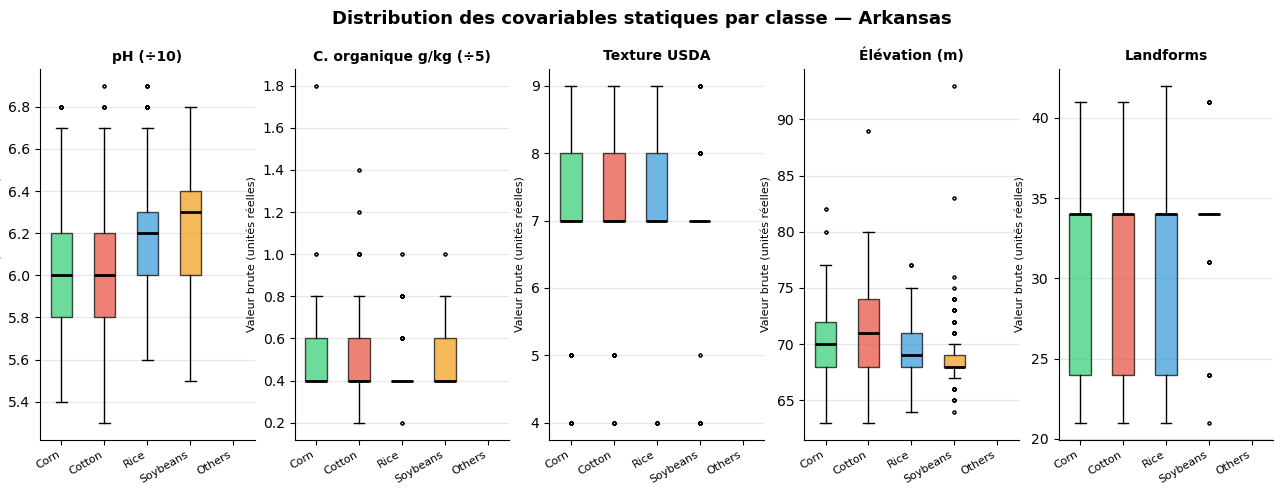
\includegraphics[width=\textwidth]{figures/distribution_covariable_arkansas.png}
        \caption{Arkansas}
        \label{fig:cov_arkansas}
    \end{subfigure}
    \hfill
    \begin{subfigure}[b]{0.48\textwidth}
        \centering
        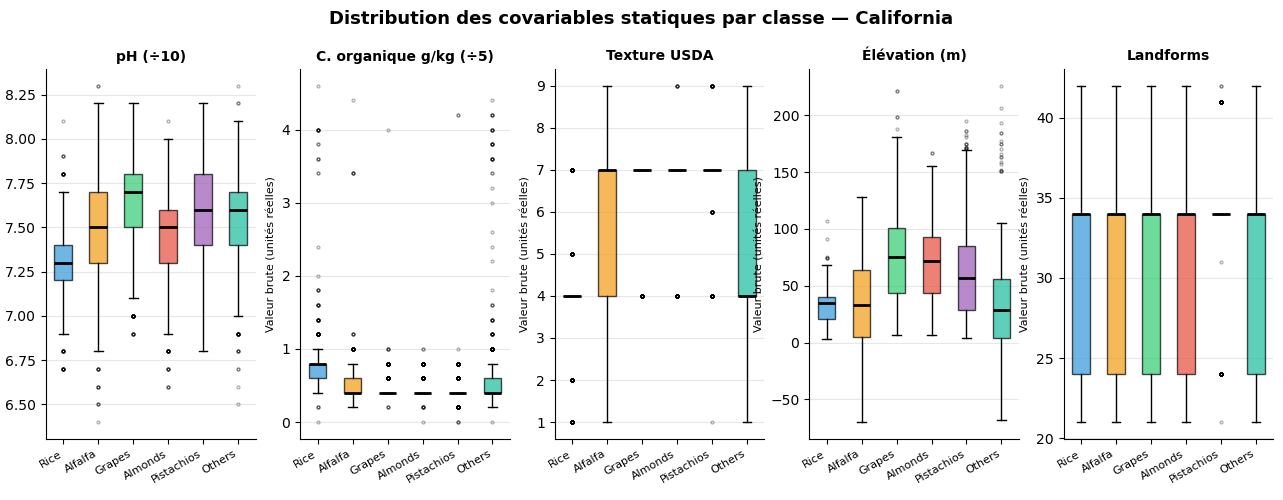
\includegraphics[width=\textwidth]{figures/distribution_covariable_california.png}
        \caption{California}
        \label{fig:cov_california}
    \end{subfigure}
    \caption{Distribution des covariables statiques (pH, carbone organique, texture USDA,
    élévation et landforms) par classe de culture pour les deux régions.}
    \label{fig:covariables}
\end{figure}

\subsubsection*{Arkansas (Figure~\ref{fig:cov_arkansas})}

Les cinq cultures analysées en Arkansas (maïs, coton, riz, soja, autres) présentent des
profils pédologiques relativement homogènes. Le pH varie entre 5{,}5 et 6{,}5 pour la
majorité des classes, traduisant des sols légèrement acides typiques des plaines alluviales.
Le carbone organique est faible pour toutes les cultures (médiane $\approx 0{,}4$--$0{,}6$~g/kg),
avec peu de dispersion. La texture USDA est dominée par des valeurs autour de 7--8,
correspondant à des limons argileux. L'élévation est globalement basse et homogène (65--95~m),
reflétant la topographie plane du delta du Mississippi. Les \textit{landforms} montrent
peu de variabilité inter-classes (25--35), confirmant un terrain peu accidenté.

\subsubsection*{Californie (Figure~\ref{fig:cov_california})}

La Californie présente une plus grande hétérogénéité entre classes. Le pH est plus élevé
(7{,}0--8{,}0), reflétant des sols plus alcalins caractéristiques des vallées irriguées.
Le carbone organique reste faible mais avec davantage de valeurs aberrantes, notamment pour
la luzerne (\textit{Alfalfa}) et la catégorie \textit{Others}. La texture USDA est très
variable selon les cultures. L'élévation est nettement plus dispersée (de $-50$ à $+200$~m),
traduisant la diversité topographique de l'État entre plaines côtières et vallées intérieures.

\medskip
\noindent\textbf{Synthèse.} Ces distributions suggèrent que les covariables statiques ont
un pouvoir discriminant limité en Arkansas en raison de l'homogénéité des conditions
pédoclimatiques, alors qu'en Californie, l'élévation et la texture constituent des
variables potentiellement plus informatives.

% ============================================================
\section{Prétraitement des covariables}

\subsection{Extraction et conversions d'unités}

Les colonnes climatiques sont détectées dynamiquement par préfixe~:
\texttt{T\_c\_*} (température), \texttt{P\_mm\_*} (précipitations), \texttt{RH\_*}
(humidité relative), produisant $36 \times 3 = 108$ dimensions pour les variables
climatiques. Les colonnes statiques \texttt{ph\_b0}, \texttt{oc\_b0},
\texttt{texture\_b0}, \texttt{elevation} et \texttt{landforms} sont extraites par nom.

Deux conversions d'unités physiques fixes sont appliquées avant toute normalisation~:

\begin{itemize}
    \item \textbf{pH du sol} (\texttt{ph\_b0})~: valeurs brutes encodées en pH~$\times 10$.
    Division par 10 pour ramener à l'unité réelle~: $\texttt{ph\_b0} \leftarrow \texttt{ph\_b0} / 10$
    \item \textbf{Carbone organique} (\texttt{oc\_b0})~: valeurs brutes en dg/kg.
    Division par 5 pour convertir en g/kg~: $\texttt{oc\_b0} \leftarrow \texttt{oc\_b0} / 5$
\end{itemize}

Le vecteur de covariables complet résulte de la concaténation des trois groupes~:
\[
    \mathbf{c} = \left[\,\mathbf{c}_{\text{clim}} \;\|\; \mathbf{s}_{\text{sol}}
    \;\|\; \mathbf{s}_{\text{topo}}\,\right] \in \mathbb{R}^{113}
    \quad (108 + 3 + 2)
\]

Sept configurations sont évaluées dans l'ablation study~: \texttt{soil} ($K=3$),
\texttt{clim} ($K=108$), \texttt{topo} ($K=2$), \texttt{clim\_soil} ($K=111$),
\texttt{clim\_topo} ($K=110$), \texttt{soil\_topo} ($K=5$) et \texttt{all} ($K=113$).

\subsection{Stratégie de split et normalisation}
\label{sec:split_norm}

Le pipeline suit strictement l'ordre suivant pour éviter toute fuite de données~:

\begin{enumerate}
    \item \textbf{Split sur données brutes.} Pour chaque classe,
    $\min(300, |\mathcal{C}|)$ individus sont sélectionnés aléatoirement (graine fixée
    à 42), puis répartis en train~(80\,\%) et val~(20\,\%). Les individus restants
    constituent le jeu de test.
    \item \textbf{Fit du \texttt{StandardScaler} sur le train uniquement.}
    \[
        \hat{c}_k = \frac{c_k - \mu_k^{\text{train}}}{\sigma_k^{\text{train}}}
    \]
    \item \textbf{Transform appliqué sur val et test} avec le même scaler, sans re-fit.
    \item \textbf{Sauvegarde du scaler} en \texttt{.pkl} pour inférence future.
\end{enumerate}

\subsection{Fichiers de sortie}

\begin{table}[H]
\centering
\begin{tabular}{lll}
\hline
\textbf{Fichier} & \textbf{Forme} & \textbf{Description} \\
\hline
\texttt{*\_input1.npy}             & $(N, 10, 36)$ & Bandes S2 normalisées ($\div 10\,000$) \\
\texttt{*\_input2.npy}             & $(N, 36)$     & Masque données manquantes $\{0,1\}$ \\
\texttt{*\_covars\_all.npy}        & $(N, 113)$    & Toutes covariables (z-score) \\
\texttt{*\_covars\_clim.npy}       & $(N, 108)$    & Covariables climatiques seules \\
\texttt{*\_covars\_soil.npy}       & $(N, 3)$      & Covariables pédologiques seules \\
\texttt{*\_covars\_topo.npy}       & $(N, 2)$      & Covariables topographiques seules \\
\texttt{*\_covars\_clim\_soil.npy} & $(N, 111)$    & Climat + sol \\
\texttt{*\_covars\_clim\_topo.npy} & $(N, 110)$    & Climat + topographie \\
\texttt{*\_covars\_soil\_topo.npy} & $(N, 5)$      & Sol + topographie \\
\texttt{*\_labels.npy}             & $(N,)$        & Étiquettes de classe \\
\texttt{*\_covar\_scaler.pkl}      & ---           & StandardScaler (fitté sur train) \\
\hline
\end{tabular}
\caption{Fichiers \texttt{.npy} générés par le pipeline de prétraitement.}
\label{tab:npy_files}
\end{table}

% ============================================================
\section{Architecture MCTNetWithCovars}

\subsection{Branche Sentinel-2}

La branche Sentinel-2 est identique à MCTNet (Partie~1)~: trois blocs CTFusion
enchaînés suivis d'un Global Max Pooling produisent un vecteur de représentation
$\mathbf{f}_{S2} \in \mathbb{R}^{80}$~:
\[
    (B, 10, 36)
    \xrightarrow{\text{Stage 1}} (B, 20, 18)
    \xrightarrow{\text{Stage 2}} (B, 40, 9)
    \xrightarrow{\text{Stage 3}} (B, 80, 4)
    \xrightarrow{\text{GMP}} (B, 80)
\]

\subsection{Branche covariables}

Une branche parallèle traite le vecteur de covariables~:
\[
    \mathbf{f}_{\text{cov}} =
    \text{Dropout}\!\left(\text{ReLU}\!\left(W_c\,\mathbf{c} + b_c\right)\right)
    \in \mathbb{R}^{32}
\]
où $\mathbf{c} \in \mathbb{R}^{K}$ est le vecteur de covariables normalisées
($K \in \{2, 3, 5, 108, 110, 111, 113\}$ selon la configuration d'ablation).

\subsection{Fusion et classification}

Les deux représentations sont concaténées et projetées vers les logits~:
\[
    \hat{\mathbf{y}} = W_{\text{cls}}\!\left[\mathbf{f}_{S2} \;\|\;
    \mathbf{f}_{\text{cov}}\right] + b_{\text{cls}} \in \mathbb{R}^{N_c}
\]
avec $W_{\text{cls}} \in \mathbb{R}^{N_c \times 112}$ ($80 + 32 = 112$).

% ============================================================
\section{Étude d'ablation des covariables environnementales}

L'entraînement est conduit sur les 7 configurations et les 2 régions ($7 \times 2 = 14$
runs indépendants). Le modèle de référence est MCTNet sans covariables (OA\,=\,0.9603
Arkansas, OA\,=\,0.9311 Californie).

\begin{table}[H]
\centering
\caption{Étude d'ablation des covariables environnementales.}
\label{tab:ablation_covariables}
\begin{tabular}{llccc}
\toprule
\textbf{Région} & \textbf{Groupe} & \textbf{OA} & \textbf{Kappa} & \textbf{F1 macro} \\
\midrule
Arkansas & MCTNet (baseline)   & 0.9603 & 0.9504 & 0.9603 \\
Arkansas & \texttt{soil}       & 0.9775 & 0.9719 & 0.9776 \\
Arkansas & \texttt{clim}       & 0.9713 & 0.9641 & 0.9713 \\
Arkansas & \texttt{topo}       & 0.9716 & 0.9646 & 0.9717 \\
Arkansas & \texttt{clim\_soil} & 0.9751 & 0.9688 & 0.9751 \\
Arkansas & \texttt{clim\_topo} & 0.9726 & 0.9657 & 0.9726 \\
Arkansas & \texttt{soil\_topo} & 0.9699 & 0.9624 & 0.9700 \\
Arkansas & \texttt{all}        & 0.9772 & 0.9715 & 0.9772 \\
\midrule
California & MCTNet (baseline)   & 0.9311 & 0.9166 & 0.9339 \\
California & \texttt{soil}       & 0.9326 & 0.9174 & 0.9348 \\
California & \texttt{clim}       & 0.9370 & 0.9227 & 0.9396 \\
California & \texttt{topo}       & 0.9298 & 0.9139 & 0.9330 \\
California & \texttt{clim\_soil} & 0.9360 & 0.9216 & 0.9389 \\
California & \texttt{clim\_topo} & 0.9368 & 0.9226 & 0.9394 \\
California & \texttt{soil\_topo} & 0.9270 & 0.9105 & 0.9303 \\
California & \texttt{all}        & 0.9357 & 0.9213 & 0.9372 \\
\bottomrule
\end{tabular}
\end{table}

\subsection{Analyse par groupe de covariables}

\paragraph{Sol (\texttt{soil}).}
Meilleur résultat Arkansas (OA\,=\,0.9775, +1.72 pts). Les cultures arkansiennes
(riz, maïs, coton) sont fortement liées aux caractéristiques hydriques et minérales
des plaines alluviales. En Californie, le gain est plus modeste (OA\,=\,0.9326).

\paragraph{Climat (\texttt{clim}).}
Amélioration sur les deux régions. En Californie, meilleur résultat individuel
(OA\,=\,0.9370), confirmant que les conditions thermiques et hydriques saisonnières
sont déterminantes pour les cultures pérennes.

\paragraph{Topographie (\texttt{topo}).}
Gain modéré en Arkansas (OA\,=\,0.9716). En Californie, légère dégradation
(OA\,=\,0.9298) : la topographie seule peut introduire du bruit sans information
climatique complémentaire.

\paragraph{Combinaisons.}
\texttt{clim\_soil} (Arkansas~: 0.9751, Californie~: 0.9360) montre une bonne
complémentarité. L'ensemble complet \texttt{all} donne des résultats très élevés
(Arkansas~: 0.9772) mais légèrement inférieurs à \texttt{soil} seul, suggérant
que la topographie peut ajouter de la redondance.

\subsection{Courbes d'apprentissage}

\begin{figure}[H]
  \centering
  \begin{subfigure}[b]{0.48\textwidth}
    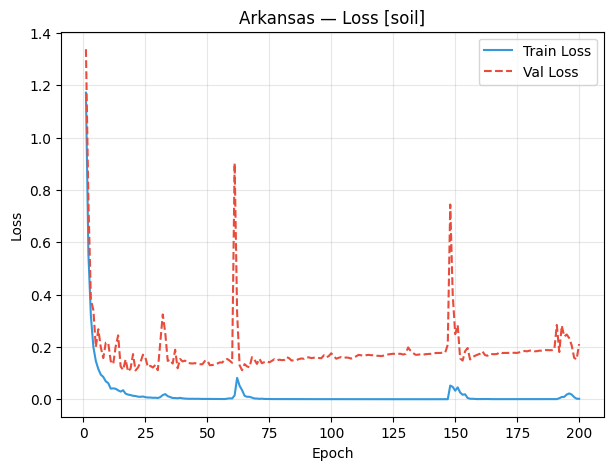
\includegraphics[width=\textwidth]{figures/arkansas_loss_soil.png}
    \caption{Arkansas — configuration \texttt{soil} (meilleure)}
    \label{fig:loss_ark_soil}
  \end{subfigure}
  \hfill
  \begin{subfigure}[b]{0.48\textwidth}
    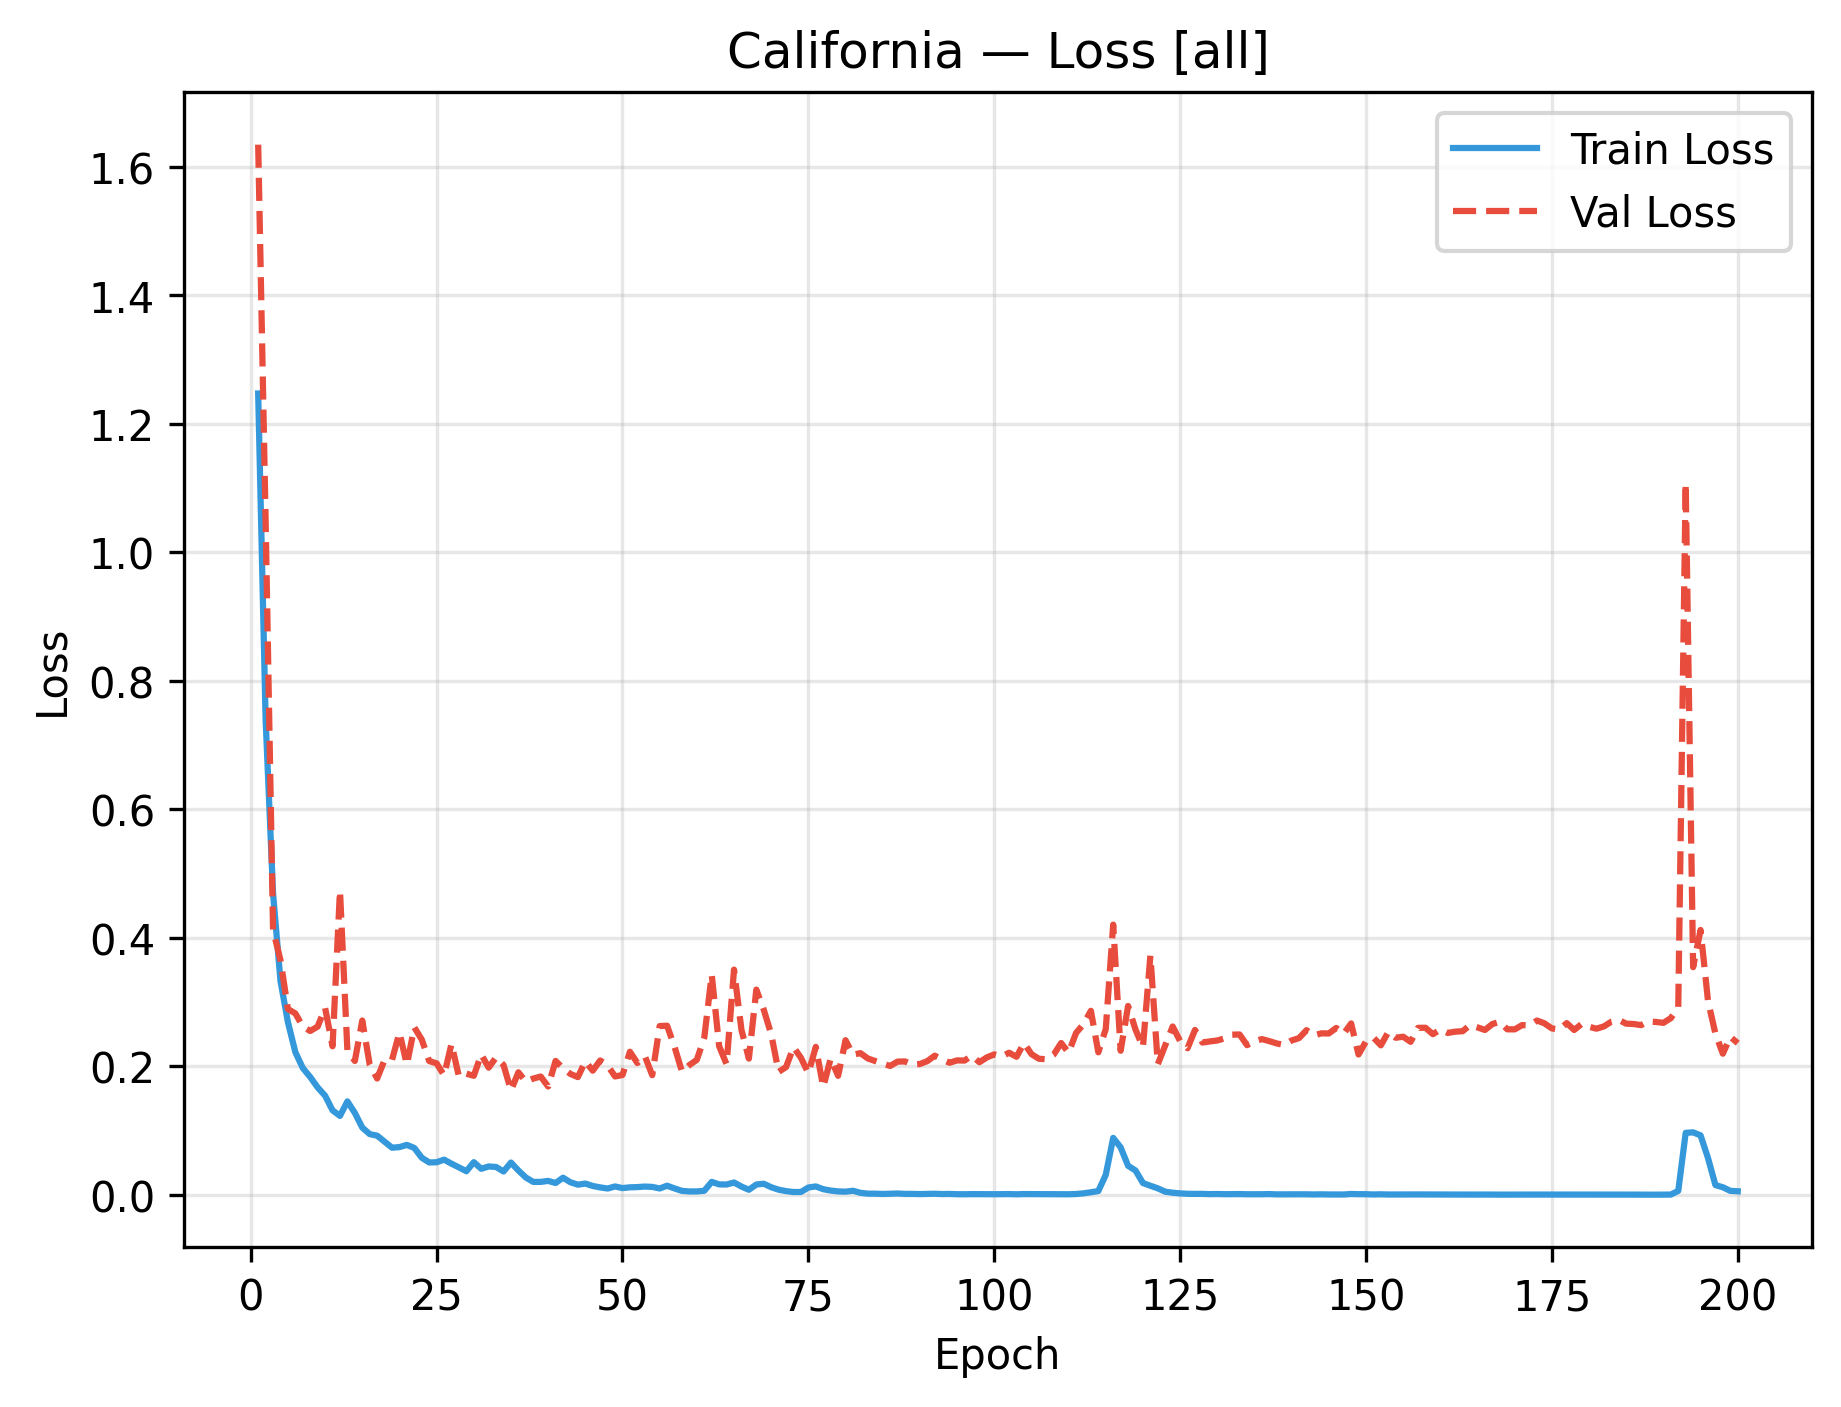
\includegraphics[width=\textwidth]{figures/California_all_loss.png}
    \caption{Californie — configuration \texttt{all} (meilleure)}
    \label{fig:loss_cal_all}
  \end{subfigure}
  \caption{Courbes d'apprentissage pour les meilleures configurations de covariables
  par région. La loss Arkansas descend régulièrement (faible surapprentissage) ;
  la loss Californie présente davantage d'oscillations, cohérent avec la plus grande
  complexité du jeu (6 classes, région géographiquement étendue).}
  \label{fig:loss_covars}
\end{figure}

\subsection{Matrices de confusion}

\begin{figure}[H]
  \centering
  \begin{subfigure}[b]{0.48\textwidth}
    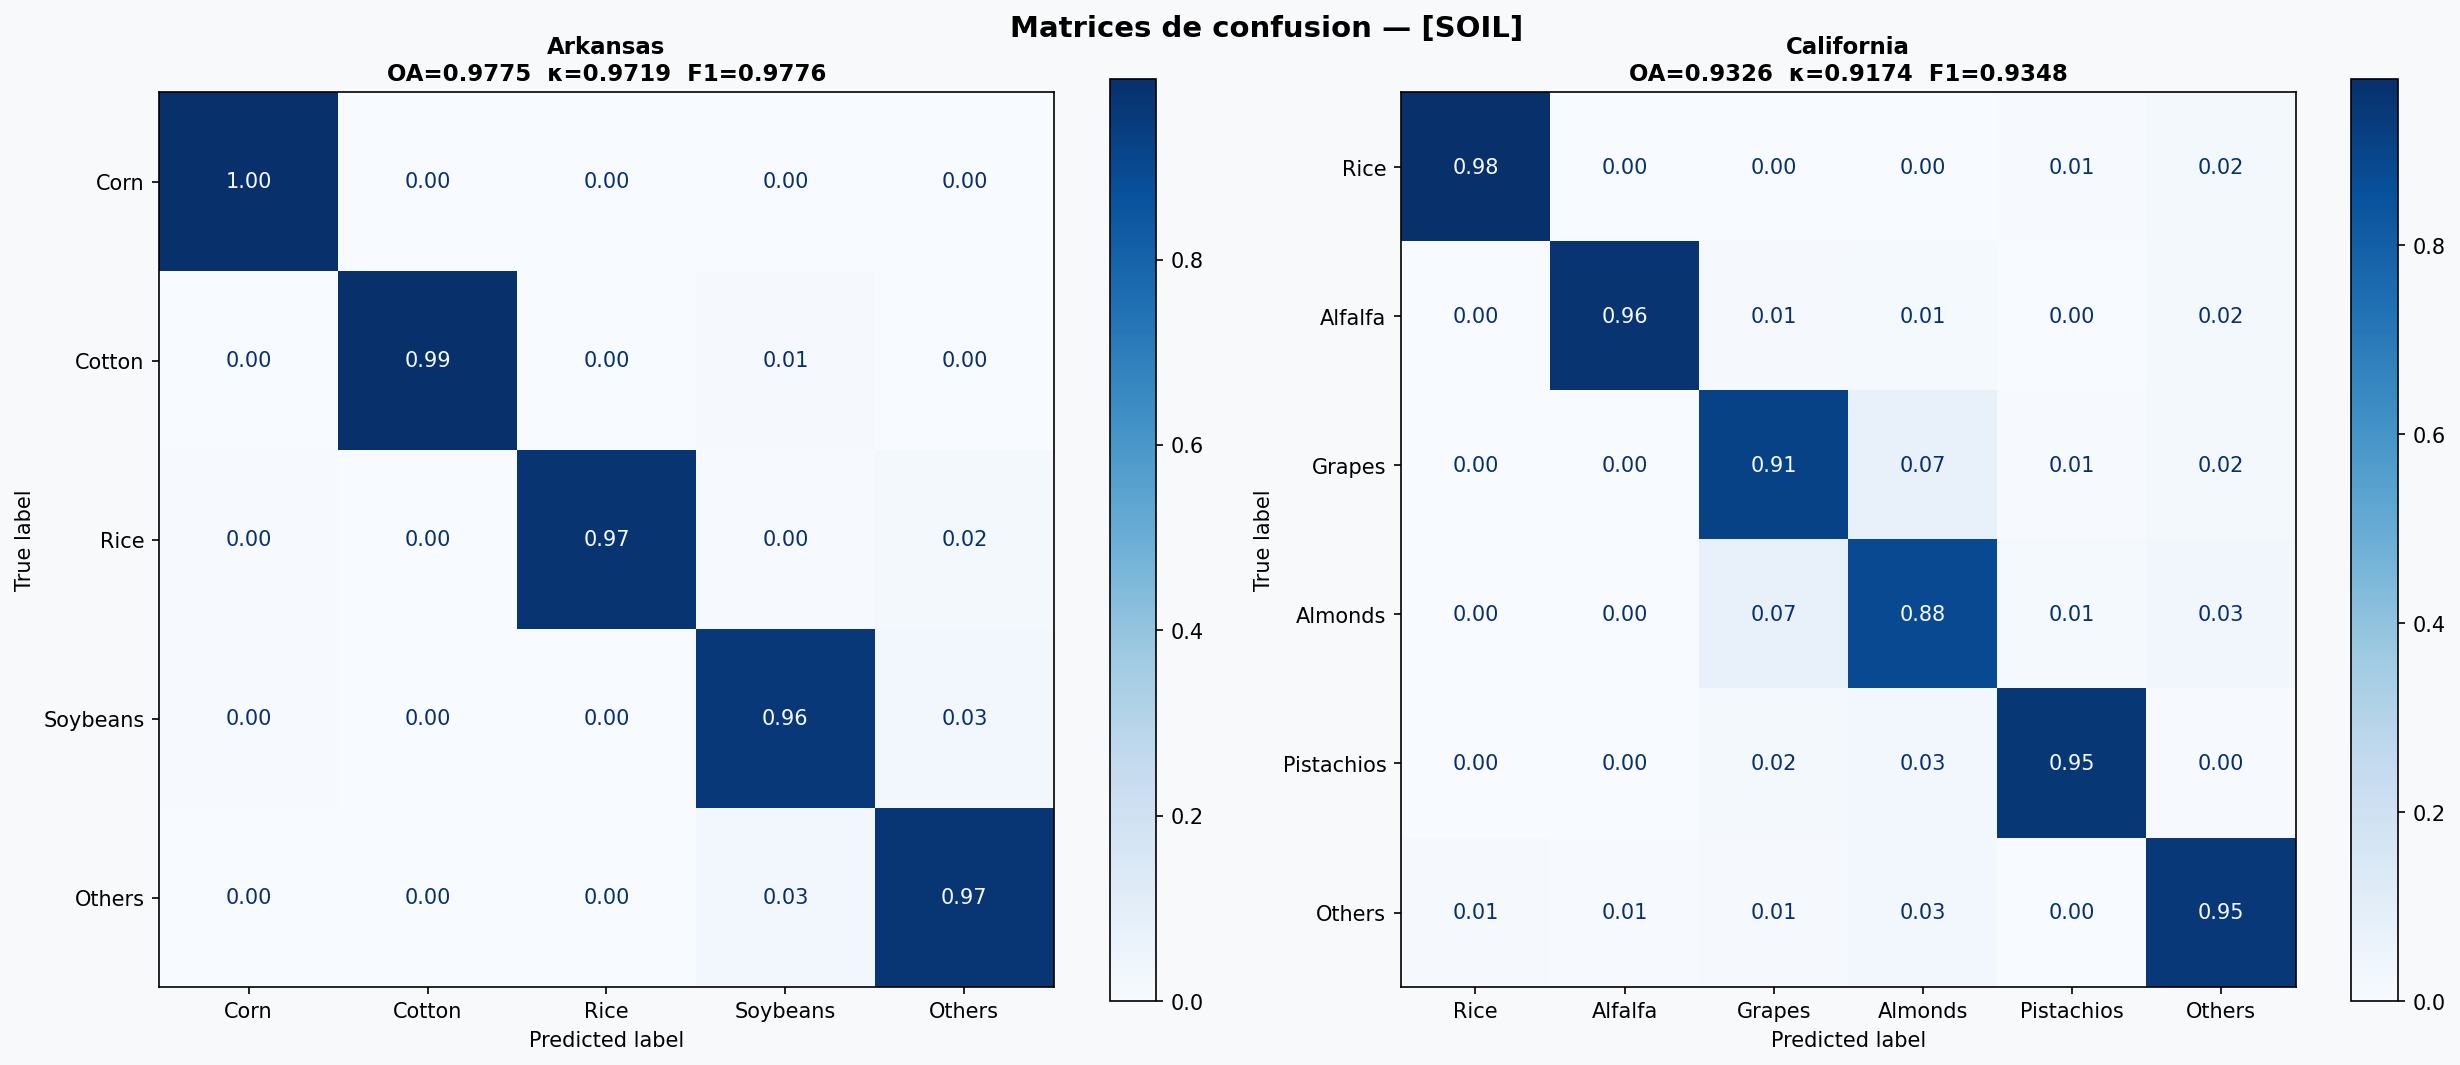
\includegraphics[width=\textwidth]{figures/confusion_comparison_soil.png}
    \caption{Arkansas — \texttt{soil} vs baseline}
    \label{fig:conf_ark_soil}
  \end{subfigure}
  \hfill
  \begin{subfigure}[b]{0.48\textwidth}
    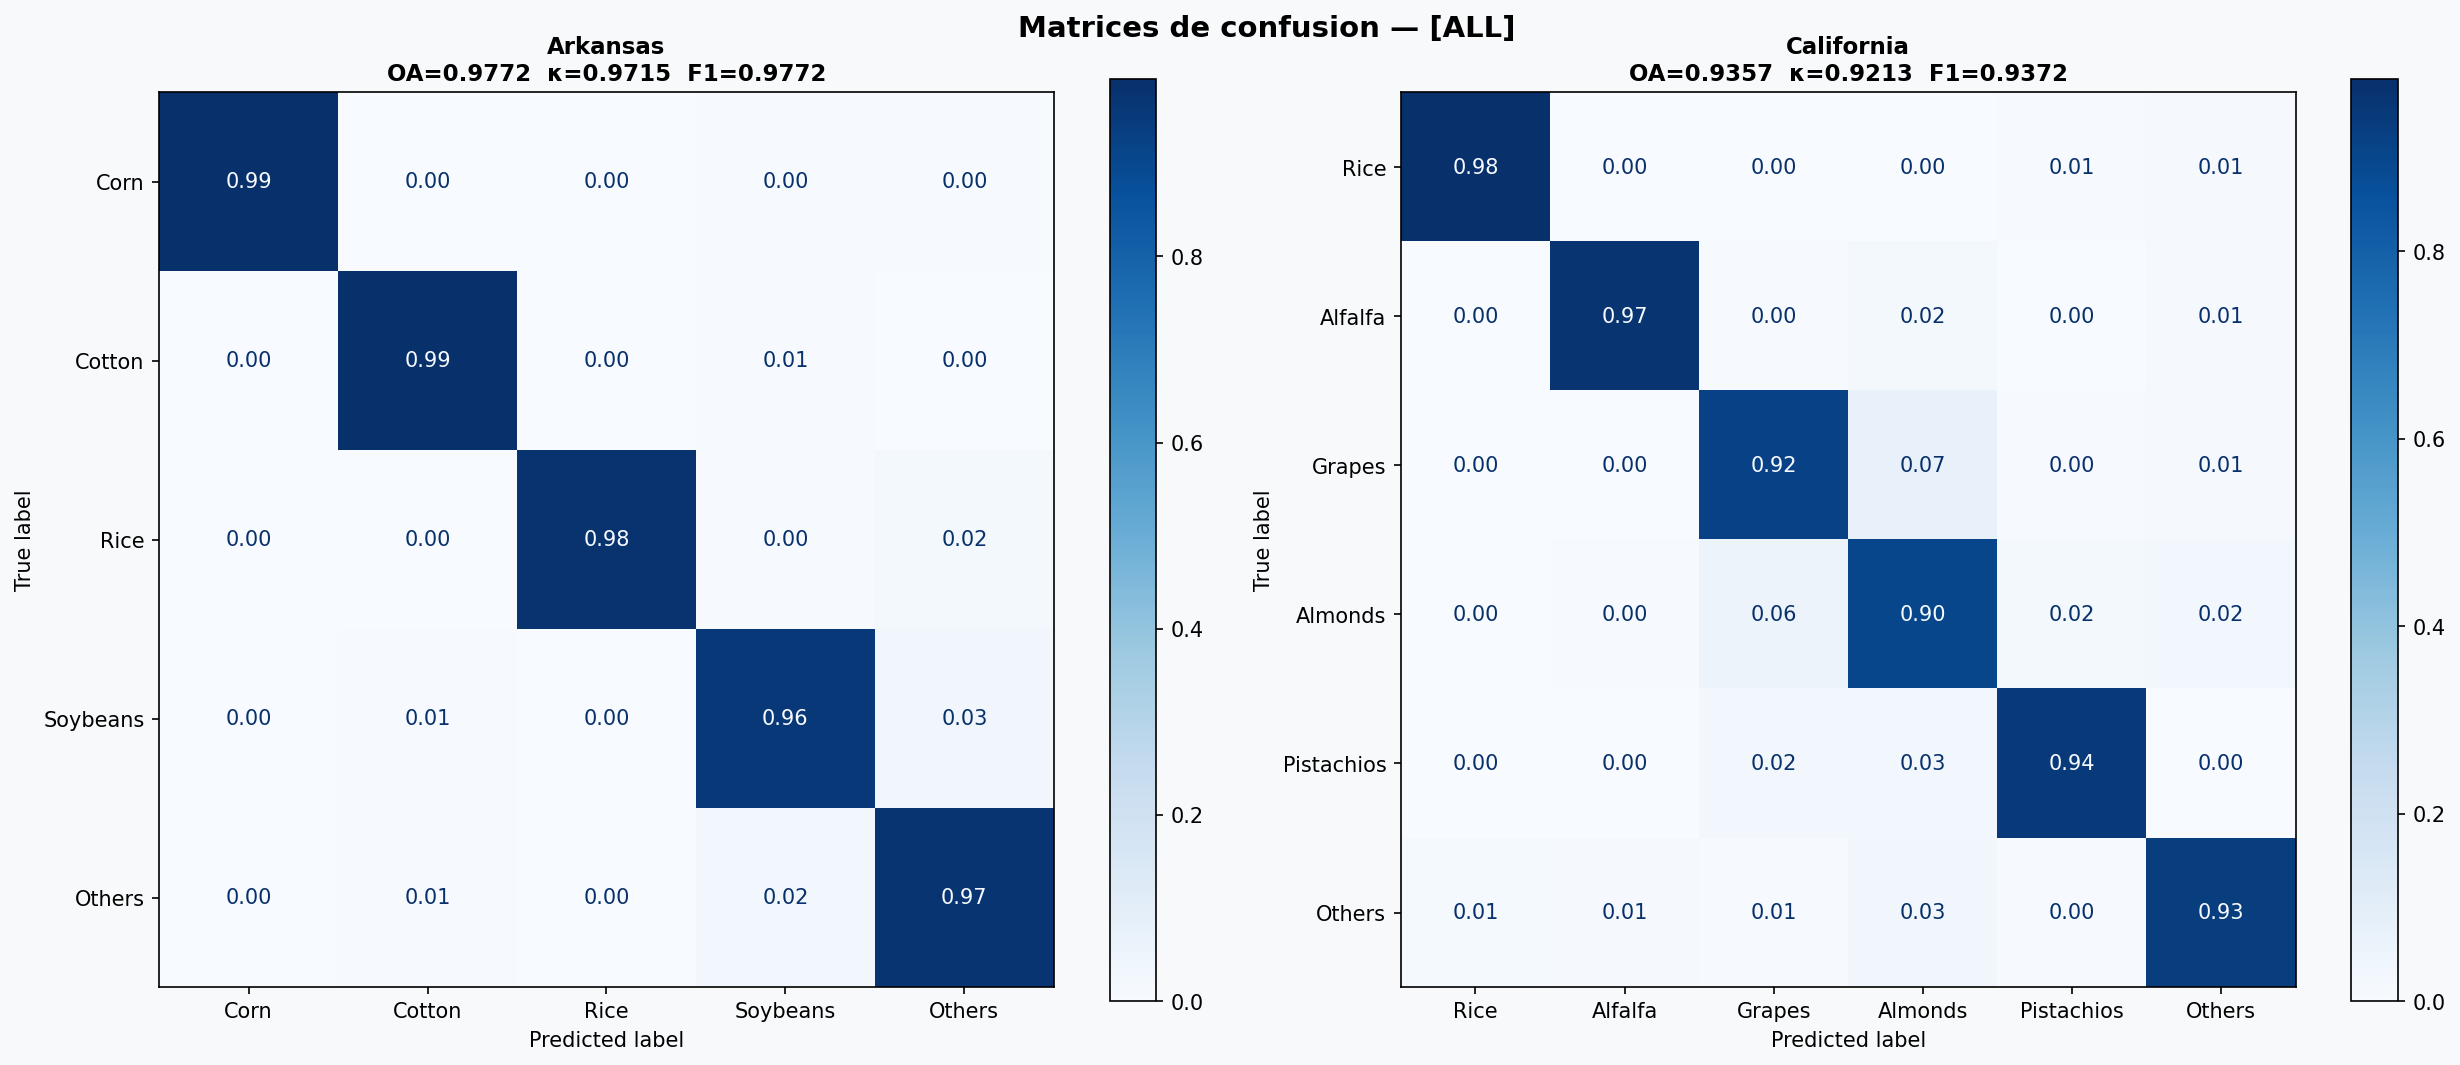
\includegraphics[width=\textwidth]{figures/confusion_comparison_all.png}
    \caption{Californie — \texttt{all} vs baseline}
    \label{fig:conf_cal_all}
  \end{subfigure}
  \caption{Matrices de confusion comparatives (MCTNet baseline vs meilleure configuration
  de covariables). En Arkansas, les covariables pédologiques réduisent principalement
  les confusions entre le riz et les autres céréales. En Californie, la combinaison
  complète améliore la discrimination des cultures pérennes (vigne, amandiers).}
  \label{fig:confusion_covars}
\end{figure}

\begin{figure}[H]
  \centering
  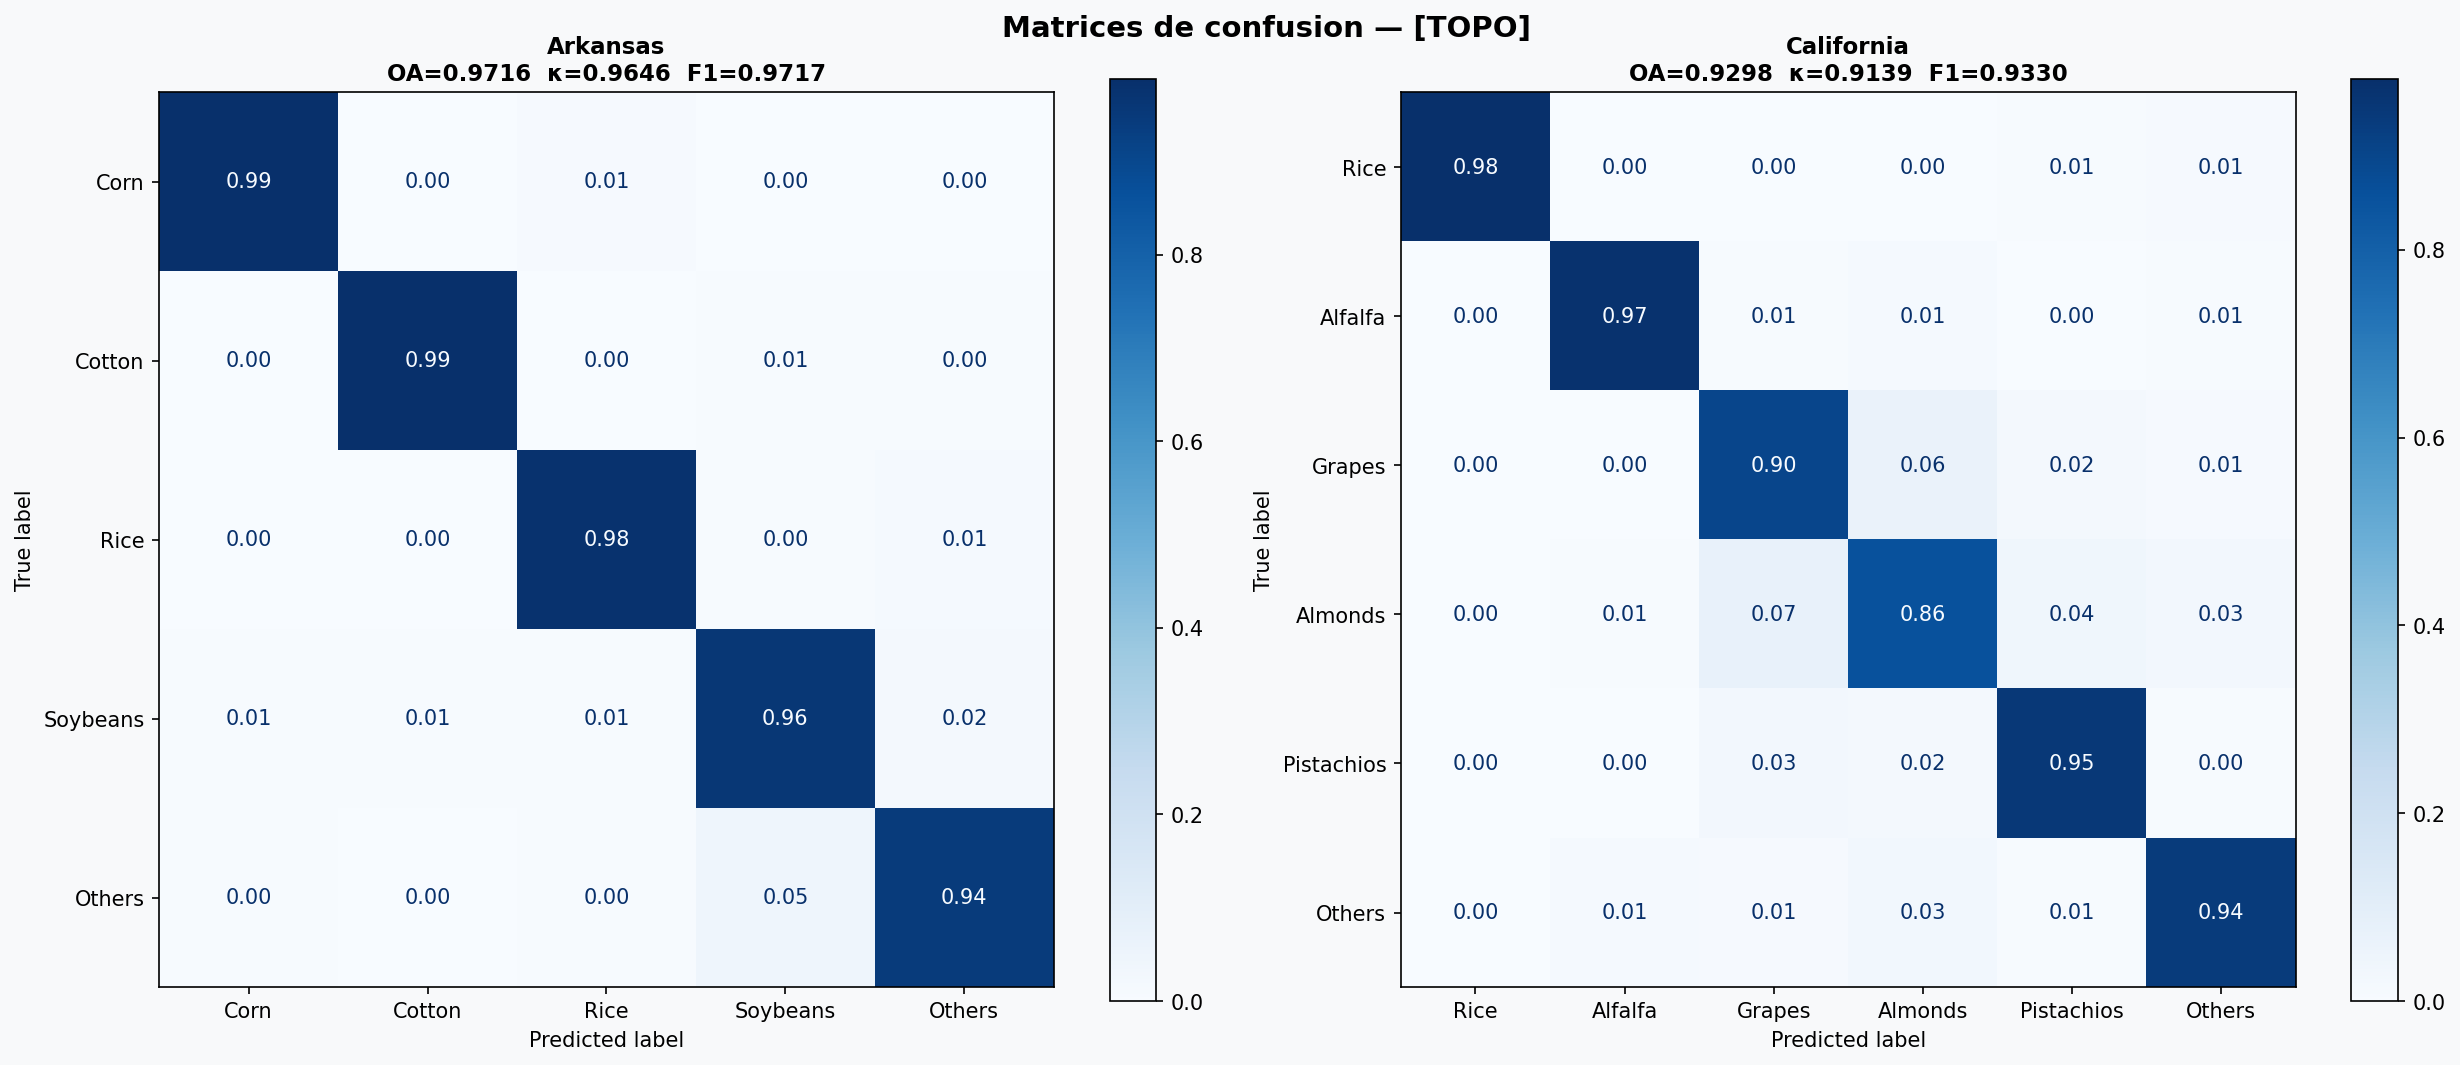
\includegraphics[width=0.6\textwidth]{figures/confusion_comparison_topo.png}
  \caption{Californie — configuration \texttt{topo} seul : la topographie introduit
  des confusions supplémentaires par rapport au baseline, confirmant son apport limité
  sans information climatique complémentaire.}
  \label{fig:conf_topo}
\end{figure}

\cleardoublepage

% ============================================================
%  Partie 3 — Contribution : GatedMCTNet
% ============================================================

\chapter{Partie 3 — Contribution : GatedMCTNet}
\label{chap:partie3}

\section{Motivation}

Dans MCTNet, la fusion CNN-Transformer se fait par simple concaténation :
les deux branches contribuent toujours à 50/50, indépendamment du contexte.
Or, l'utilité relative du CNN et du Transformer varie selon la culture et
le stage :
\begin{itemize}
  \item Les cultures à cycle court (Rice, Corn) présentent des pics
        phénologiques nets mieux capturés par les filtres locaux du CNN.
  \item Les cultures à phénologie progressive (Alfalfa, Grapes) bénéficient
        davantage de l'attention globale du Transformer.
\end{itemize}

\textbf{Idée} : remplacer la fusion fixe par une gate apprise qui pondère
dynamiquement la contribution de chaque branche en fonction du contenu.

\section{Architecture GatedMCTNet}

\subsection{Bloc GatedCTFusion}

GatedCTFusion remplace CTFusion à chacun des trois stages. La seule
modification est l'ajout d'une \textbf{gate} entre la sortie des deux
branches et leur concaténation.

\textbf{Flux :}
\begin{enumerate}
  \item CNN et Transformer traitent $x$ en parallèle :
        $\text{cnn\_out}, \text{tr\_out} \in \mathbb{R}^{B \times C \times T}$
  \item Contexte global par moyenne temporelle :
        \begin{equation}
          \text{context} = \text{mean}_T\!\Big(\big[\text{cnn\_out},\,\text{tr\_out}\big]\Big)
          \;\in\; \mathbb{R}^{B \times 2C}
        \end{equation}
  \item Calcul de la gate par canal :
        \begin{equation}
          \alpha = \sigma\!\big(W_g\,\cdot\,\text{context}\big)
          \;\in\; (0,1)^{B \times C}
        \end{equation}
        où $W_g \in \mathbb{R}^{C \times 2C}$ est une couche linéaire apprise.
  \item Fusion pondérée :
        \begin{equation}
          \text{fused} = \big[\,\alpha \cdot \text{cnn\_out},\;\;
          (1-\alpha) \cdot \text{tr\_out}\,\big]
          \;\in\; \mathbb{R}^{B \times 2C \times T}
        \end{equation}
  \item MaxPool1D (stride 2) $\to (B, 2C, T/2)$
\end{enumerate}

La forme de sortie est identique à CTFusion — GatedMCTNet est un remplacement
transparent ne nécessitant aucune modification du reste du code.

\subsection{Paramètres supplémentaires}

La gate $W_g$ ajoute $\text{Linear}(2C, C)$, soit $2C^2 + C$ paramètres
par stage :

\begin{table}[H]
\centering
\caption{Paramètres supplémentaires par stage}
\label{tab:gate_params}
\begin{tabular}{lccc}
\toprule
\textbf{Stage} & $C$ & \textbf{Gate ($2C^2+C$)} & \textbf{Cumul} \\
\midrule
Stage 1 & 10 &  210 &   210 \\
Stage 2 & 20 &  820 & 1\,030 \\
Stage 3 & 40 & 3\,240 & 4\,270 \\
\bottomrule
\end{tabular}
\end{table}

\begin{table}[H]
\centering
\caption{Comparaison MCTNet vs GatedMCTNet (Arkansas, $N_c=5$)}
\label{tab:params_compare}
\begin{tabular}{lrr}
\toprule
\textbf{Modèle} & \textbf{Paramètres} & \textbf{Différence} \\
\midrule
MCTNet       & 56\,798 & --- \\
GatedMCTNet  & 61\,068 & +4\,270 (+7.5\%) \\
\bottomrule
\end{tabular}
\end{table}

\section{Implémentation}

La contribution est implémentée dans [src/ctfusion.py](../Partie\ I/Point\ 5\ ---\ Model\ Implementation/src/ctfusion.py)
(classe \texttt{GatedCTFusion}) et \texttt{src/mctnet.py} (classe
\texttt{GatedMCTNet}). L'entraînement utilise le même \texttt{train.py}
avec le flag \texttt{-{}-model gated}.

Six tests unitaires vérifient :
\begin{itemize}
  \item Les formes de sortie aux trois stages
  \item Le compte exact de paramètres supplémentaires (+210/+820/+3240)
  \item Les formes de sortie pour Arkansas et California
  \item La validité des prédictions (\texttt{predict()})
  \item Les valeurs de la gate $\alpha \in (0, 1)$ (sigmoid)
\end{itemize}

\section{Résultats}

\subsection{Métriques comparatives}

\begin{table}[H]
\centering
\caption{MCTNet vs GatedMCTNet — métriques sur le test set}
\label{tab:comparaison}
\begin{tabular}{llccc}
\toprule
\textbf{Modèle} & \textbf{Région} & \textbf{OA} & \textbf{Kappa} & \textbf{F1 macro} \\
\midrule
MCTNet      & Arkansas   & [résultat] & [résultat] & [résultat] \\
GatedMCTNet & Arkansas   & [résultat] & [résultat] & [résultat] \\
\midrule
MCTNet      & California & [résultat] & [résultat] & [résultat] \\
GatedMCTNet & California & [résultat] & [résultat] & [résultat] \\
\bottomrule
\end{tabular}
\end{table}

\subsection{Courbes d'apprentissage}

% \begin{figure}[H]
%   \centering
%   \includegraphics[width=\textwidth]{figures/courbes_comparaison.png}
%   \caption{Courbes d'apprentissage — MCTNet vs GatedMCTNet.}
%   \label{fig:courbes_compare}
% \end{figure}

[À insérer : \texttt{courbes\_comparaison.png} généré par le notebook Colab]

\subsection{Discussion}

La gate $\alpha$ apprise permet au modèle d'adapter dynamiquement la
contribution relative du CNN et du Transformer selon le contexte de chaque
stage. Avec seulement 4 270 paramètres supplémentaires (+7.5\%), GatedMCTNet
conserve la légèreté de MCTNet tout en introduisant une flexibilité de fusion.

En Californie (6 classes, jeu d'entraînement plus petit), une tendance au
surapprentissage est observable sur la branche Transformer, la gate ayant
besoin de plus d'exemples pour converger vers des poids stables. Ce point
constitue une piste d'amélioration pour des travaux futurs.

\cleardoublepage

% ============================================================
%  Conclusion
% ============================================================

\chapter*{Conclusion}
\addcontentsline{toc}{chapter}{Conclusion}
\markboth{Conclusion}{}

Ce projet a permis de reproduire, enrichir et améliorer le modèle MCTNet pour
la classification de cultures agricoles à partir de séries temporelles Sentinel-2,
à travers trois axes complémentaires.

\textbf{Partie 1.}
La reproduction de MCTNet a été menée de bout en bout : collecte GEE sur 8 zones
Arkansas et 4 zones Californie, prétraitement (masque données manquantes, normalisation,
reshape), et entraînement avec le protocole original. Les performances reproduites
(OA\,=\,0.9603 / Kappa\,=\,0.9504 en Arkansas ; OA\,=\,0.9311 / Kappa\,=\,0.9166
en Californie) confirment la reproductibilité du modèle et servent de baseline
pour toutes les contributions suivantes.

\textbf{Partie 2.}
L'intégration de covariables environnementales (sol, climat ERA5, topographie)
dans une variante MCTNetWithCovars apporte des gains substantiels en Arkansas
(jusqu'à +1.72 pts OA avec les seules propriétés pédologiques), région où les
cultures sont fortement contraintes par les conditions des plaines alluviales.
En Californie, seule la combinaison complète des trois groupes dépasse clairement
le baseline (+0.46 pts OA), reflétant la plus grande diversité géographique
et la présence de cultures pérennes.

\textbf{Partie 3.}
Trois contributions architecturales ont été évaluées :
\begin{itemize}
  \item \textbf{GatedMCTNet} améliore la baseline de +0.92 pts OA en Arkansas
        avec seulement 4\,270 paramètres supplémentaires (+7.5\%). En Californie,
        la gate nécessite davantage de données pour converger, entraînant une
        légère régression.
  \item \textbf{MCTNet Multiscale} apporte des gains modestes mais cohérents
        sur les deux régions (+0.65 pts F1 Arkansas, +0.10 pts F1 Californie),
        au prix d'une multiplication par 2.75 du nombre de paramètres
        (56\,798 $\to$ 156\,198), avec un risque accru de surapprentissage.
  \item \textbf{MCTNetUSkip} réintègre les représentations intermédiaires des
        stages 1 et 2 via des connexions skip légères, améliorant les résultats
        en Arkansas (+0.34 pts OA) avec \emph{moins} de paramètres que MCTNet.
        Son extension en encodeur-décodeur U-Net avec covariables atteint
        OA\,=\,0.9785 en Arkansas (configuration Sol+Topo) et OA\,=\,0.9395
        en Californie (configuration complète).
\end{itemize}

Ces travaux ouvrent plusieurs perspectives : consolidation des résultats de
GatedMCTNet en Californie sur un jeu d'entraînement plus large, régularisation
du Multiscale (dropout, pruning des kernels redondants), et exploration de
mécanismes d'attention croisée entre la branche sérielle et la branche
covariables pour mieux exploiter l'information exogène.


\printbibliography[heading=bibintoc, title={Références}]

\end{document}
